\documentclass[12pt,addpoints]{evalua}
\grado{1$^\circ$ de Secundaria}
\cicloescolar{2023-2024}
\materia{Matemáticas 1}
\unidad{3}
\title{Examen de la Unidad}
\aprendizajes{\footnotesize%
    \item Verifica algebraicamente la equivalencia de expresiones de primer grado, formuladas a partir de sucesiones.
    \item Resuelve problemas mediante la formulación y solución algebraica de ecuaciones lineales.
    \item Usa e interpreta las medidas de tendencia central (moda, media aritmética y mediana).
    \item Calcula el área y volumen de piramides, prismas y cilindros rectos.
    \item Calcula el perímetro y el área de polígonos regulares y del círculo a partir de diferentes datos.
    }
     \author{Prof.: Julio César Melchor Pinto}
\begin{document}
\begin{questions}
      % \section*{\ifprintanswers   {Sucesiones}\else{}\fi}
      % \subsection*{\ifprintanswers{Completa la sucesión aritmética 1}\else{}\fi}

      \question[6]{Escribe los términos faltantes de las siguientes sucesiones aritméticas:

            \begin{multicols}{3}
                  \begin{parts}
                        \part 28, 39, 50, \fillin[61][0.5cm], \fillin[72][0.5cm], \fillin[84][0.5cm], \dots
                        \part 56, 50, 44, \fillin[38][0.5cm], \fillin[32][0.5cm], \fillin[26][0.5cm], \dots
                        \part 33, 41, 49, \fillin[57][0.5cm], \fillin[65][0.5cm], \fillin[73][0.5cm], \dots
                  \end{parts}
            \end{multicols}
      }

      % \subsection*{\ifprintanswers{Completa la sucesión aritmética 2}\else{}\fi}

      \question[6]{Escribe los primeros 4 términos de las siguientes sucesiones aritméticas:

            \begin{multicols}{3}
                  \begin{parts}
                        \part
                        \[a_n=7n+4\] \fillin[11][0.5cm], \fillin[18][0.5cm], \fillin[25][0.5cm], \fillin[32][0.5cm], \dots
                        % \part $-2n+4$ \hfill \fillin[2][0.5cm], \fillin[0][0.5cm], \fillin[-2][0.5cm], \fillin[-4][0.5cm], \dots
                        \part
                        \[a_n=-5n+15 \]  \fillin[10][0.5cm], \fillin[5][0.5cm], \fillin[0][0.5cm], \fillin[-5][0.5cm], \dots
                        \part
                        \[a_n=-n-5\]   \fillin[-6][0.5cm], \fillin[-7][0.5cm], \fillin[-8][0.5cm], \fillin[-9][0.5cm], \dots
                  \end{parts}
            \end{multicols}
      }

      % \subsection*{\ifprintanswers{Completa la sucesión geométrica}\else{}\fi}

      \question[6]{Escribe los términos faltantes de las siguientes sucesiones geométricas

            \begin{multicols}{3}
                  \begin{parts}
                        \part 12, 60, \fillin[300][0.5cm], \fillin[1500][0.5cm], \fillin[7500][0.5cm], \dots
                        \part 10, 20, \fillin[40][0.5cm], \fillin[80][0.5cm], \fillin[160][0.5cm], \dots
                        \part 2, 4, 8 \fillin[16][0.5cm], \fillin[32][0.5cm], \fillin[64][0.5cm], \dots
                  \end{parts}
            \end{multicols}
      }


      % \subsection*{\ifprintanswers{Diferencia de una sucesión}\else{}\fi}

      \question[6]{Determina la diferencia de las siguientes sucesiones aritméticas

            \begin{multicols}{3}
                  \begin{parts}
                        \part 14, 12, 10, 8, 6, \dots \\[1em]
                        d=\fillin[-2][1cm]
                        \part 33, 27, 21, 15, 9, \dots \\[1em]
                        d=\fillin[-6][1cm]
                        \part -10, -8, -6, -4,  \dots \\[1em]
                        d=\fillin[2][1cm]
                  \end{parts}
            \end{multicols}
      }

      \newpage

      % \subsection*{\ifprintanswers{Término de una sucesión}\else{}\fi}
      \question[4]{Contesta las siguientes preguntas:

            \begin{multicols}{2}
                  \begin{parts}
                        \part ¿Cuál es el término 29 de la siguiente sucesión?
                        \[a_{n}=12n+24\]
                        \begin{solutionbox}{2cm}
                        \end{solutionbox}

                        \part ¿Cuál es el término 41 de la siguiente sucesión?
                        \[  a_{n}=5n+5\]
                        \begin{solutionbox}{2cm}
                        \end{solutionbox}
                  \end{parts}
            \end{multicols}
      }

      % \section*{\ifprintanswers   {Proporcionalidad y estadística}\else{}\fi}
      % \subsection*{\ifprintanswers{Razones y proporciones}\else{}\fi}

      \question[8]{Resuelve los siguientes problemas:

            \begin{multicols}{2}
                  \begin{parts}
                        \part Si la razón entre niños y niñas en un salón es de 2 a 3, ¿cuántas niñas habrá en un salón en donde hay 25 personas?
                        \fillin[10][2cm]
                        \begin{solutionbox}{1.5cm}
                        \end{solutionbox}

                        \part El costo de un kilo de aguacate es de 68 pesos, ¿cuánto se pagará por cinco cajas que cada una tiene 16 kilos de aguacate?
                        \fillin[5440][2cm]
                        \begin{solutionbox}{1.5cm}
                        \end{solutionbox}

                        %         \end{parts}
                        %     \end{multicols}
                        % }


                        % % \subsection*{\ifprintanswers{Variación directa e inversa}\else{}\fi}

                        % \question[4]{Contesta las siguientes preguntas:

                        %     \begin{multicols}{2}
                        %         \begin{parts}
                        \part En un día de trabajo de 8 horas, un obrero ha hecho 10 cajas, ¿cuántas horas tardarán en hacer 30 cajas?
                        \fillin[24][2cm]
                        \begin{solutionbox}{1.5cm}
                        \end{solutionbox}

                        \part Un camión que viaja a 60 kilómetros por hora tarda 40 minutos en cubrir cierto recorrido, ¿cuánto tardará un coche que viaja a 150 kilómetros por hora?
                        \fillin[16][2cm]
                        \begin{solutionbox}{1.5cm}
                        \end{solutionbox}

                  \end{parts}
            \end{multicols}
      }


      % \subsection*{\ifprintanswers{Mediana y moda}\else{}\fi}

      \question[4]{Contesta las siguientes preguntas:

            \begin{multicols}{2}
                  \begin{parts}
                        \part Las calificaciones de un salón de secundaria son las siguientes: 80, 82, 85, 88, 90, 88, 91, 85, 95, 88, 88, 97, 100. ¿Cuál es la mediana de las calificaciones?
                        \fillin[88][2cm]
                        \begin{solutionbox}{2cm}
                        \end{solutionbox}

                        \part Las edades de un grupo de personas son: 44, 41, 47, 48, 44, 39, 45, 49, 44 y 47 años. ¿Cuál es la mediana de las edades?
                        \fillin[44.5][2cm]
                        \begin{solutionbox}{2cm}
                        \end{solutionbox}

                  \end{parts}
            \end{multicols}
      }

      \question[6]{En mi colegio entre alumnos y alumnas somos 418. Si el número de chicas supera en 42 al de chicos, ¿cuántos alumnos y alumnas hay?

            \begin{solutionbox}{1.5cm}
            \end{solutionbox}
      }

      \newpage

      % \subsection*{\ifprintanswers{Promedio}\else{}\fi}

      \question[4]{Contesta las siguientes preguntas:

            \begin{multicols}{2}
                  \begin{parts}
                        \part El número de goles en las últimas 3 temporadas de un delantero fueron: 22, 26 y 31, ¿cuál es el promedio de goles por temporada?
                        \fillin[26.33][2cm]
                        \begin{solutionbox}{2cm}
                        \end{solutionbox}

                        \part En un grupo de 11 personas se registraron los siguientes pesos: 62, 64, 65, 59, 68, 72, 77, 71, 82, 69 y 76 kg. ¿Cuál es el promedio de los pesos?
                        \fillin[69.54][2cm]
                        \begin{solutionbox}{2cm}
                        \end{solutionbox}

                  \end{parts}
            \end{multicols}
      }

      % \subsection*{\ifprintanswers{Interpretación de gráficas}\else{}\fi}

      \question[3]{Los resultados de una encuesta se muestran en la siguiente gráfica de barras:


            De acuerdo con la gráfica,
            \begin{multicols}{2}
                  \begin{parts}
                        \part  ¿cuántas personas participaron en la encuesta? \fillin[95][2cm]
                        \part  ¿cuál es la fruta menos preferida por las personas? \fillin[Naranja][2cm]
                        \part  ¿cuál es la fruta preferida por las personas? \fillin[Manzana][2cm]

                        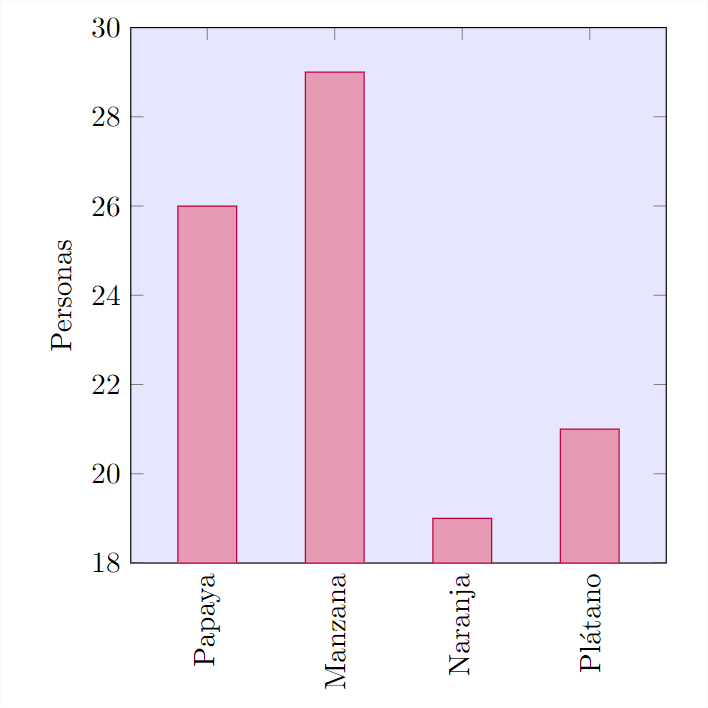
\includegraphics[width=.9\linewidth]{mexmat00001.png}
                  \end{parts}
            \end{multicols}
      }

      % \newpage

      % \section*{\ifprintanswers   {Círculo}\else{}\fi}
      % \subsection*{\ifprintanswers{Diámetro de un círculo}\else{}\fi}
      % \subsection*{\ifprintanswers{Radio de un círculo}\else{}\fi}
      % \subsection*{\ifprintanswers{Perímetro}\else{}\fi}
      % \subsection*{\ifprintanswers{Área}\else{}\fi}

      \question[9]{ Calcula el perímetro y área de los siguientes círculos:

            \begin{multicols}{3}
                  \begin{parts}
                        \part 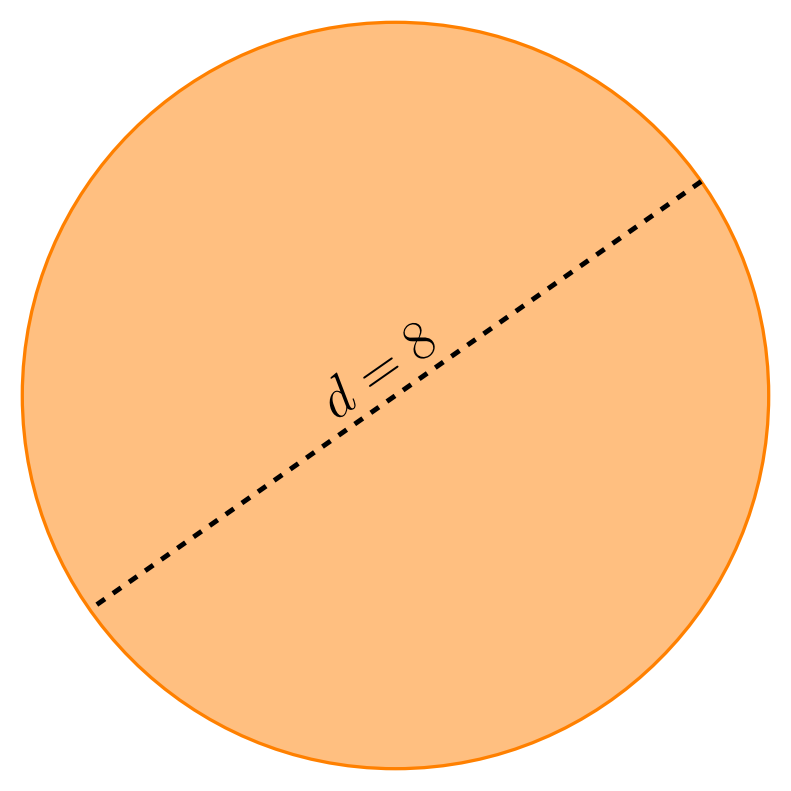
\includegraphics[width=0.9\linewidth]{mexmat00002.png}\\
                        Perímetro: \fillin[][0.3in] \quad Área: \fillin[][0.3in]

                        \begin{solutionbox}{1.5cm}
                        \end{solutionbox}

                        \part 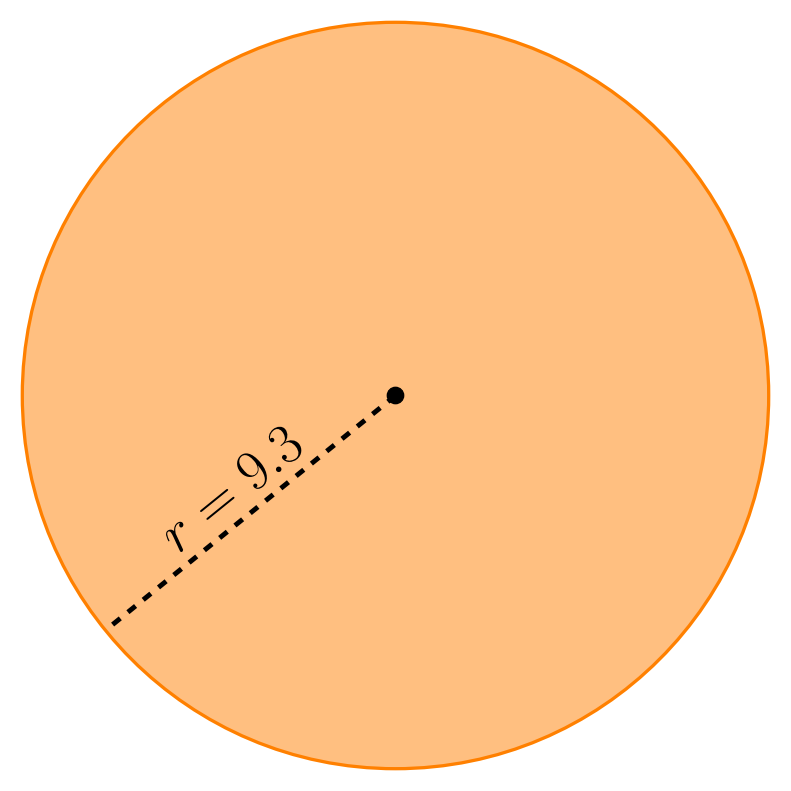
\includegraphics[width=0.9\linewidth]{mexmat00003.png}\\
                        Perímetro: \fillin[][0.3in] \quad Área: \fillin[][0.3in]

                        \begin{solutionbox}{1.5cm}
                        \end{solutionbox}

                        \part 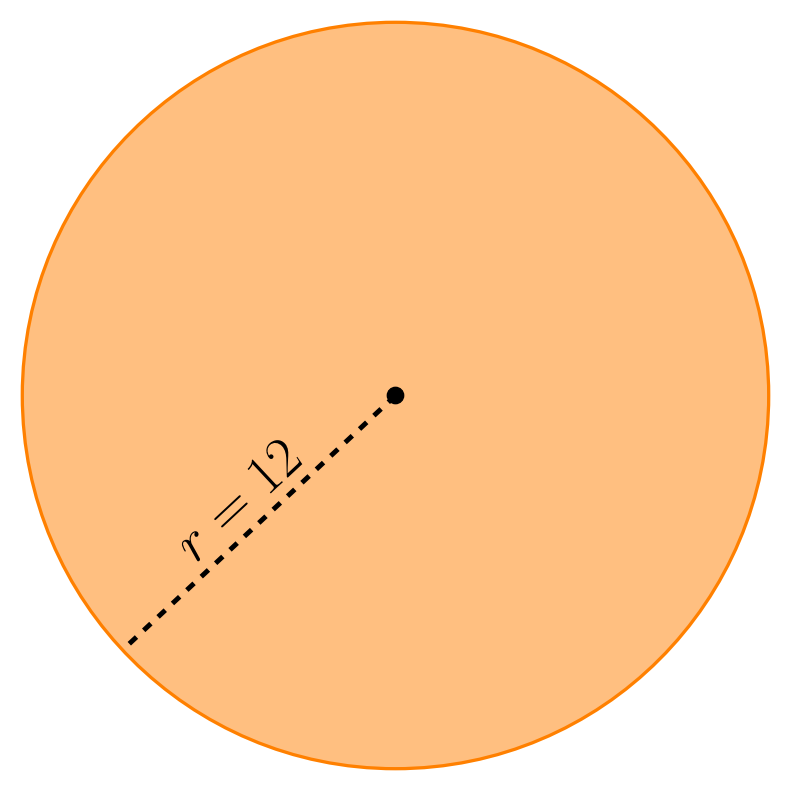
\includegraphics[width=0.9\linewidth]{mexmat00004.png}\\
                        Perímetro: \fillin[][0.3in] \quad Área: \fillin[][0.3in]

                        \begin{solutionbox}{1.5cm}
                        \end{solutionbox}
                  \end{parts}
            \end{multicols}

      }

      % \subsection*{\ifprintanswers{Resolución de problemas}\else{}\fi}

      \question[4]{Contesta las siguientes preguntas:

            \begin{multicols}{2}
                  \begin{parts}
                        \part Lisa tiene un terreno circular con un radio de 8 metros al cual le desea poner una barda en su periferia, si el precio por metro de barda es de 56 pesos. ¿Cuánto pagará en total por poner la barda?
                        \$\fillin[2813.44][2cm]

                        \begin{solutionbox}{1.5cm}
                        \end{solutionbox}

                        \part Rodolfo quiere pintar una plataforma circular de 8 metros de radio, si el costo por pintar un metro cuadrado es de 98 pesos. ¿Cuánto pagará en total Rodolfo por pintar toda la plataforma?
                        \$\fillin[19694.08][2cm]

                        \begin{solutionbox}{1.5cm}
                        \end{solutionbox}

                  \end{parts}
            \end{multicols}
      }

      % \section*{\ifprintanswers   {Ecuaciones}\else{}\fi}
      % \subsection*{\ifprintanswers{Lenguaje algebraico}\else{}\fi}

      \question[4]{Escribe la expresión algebraica correcta para los siguientes enunciados:

            \begin{multicols}{2}
                  \begin{parts}
                        \part El doble del cuadrado de un número.

                        \begin{solutionbox}{1cm}
                        \end{solutionbox}

                        \part El cuadrado de la suma de dos números.

                        \begin{solutionbox}{1cm}
                        \end{solutionbox}
                  \end{parts}
            \end{multicols}
      }

      % \subsection*{\ifprintanswers{Ecuaciones x+a=b}\else{}\fi}

      \question[6]{Resuelve las siguientes ecuaciones:

            \begin{multicols}{3}
                  \begin{parts}
                        \part \[ x+7=12 \]

                        \begin{solutionbox}{1.5cm}
                        \end{solutionbox}

                        \part \[ x+182=-199 \]

                        \begin{solutionbox}{1.5cm}
                        \end{solutionbox}

                        \part \[ x-14=34 \]

                        \begin{solutionbox}{1.5cm}
                        \end{solutionbox}
                  \end{parts}
            \end{multicols}
      }

      % \subsection*{\ifprintanswers{Ecuaciones ax=b}\else{}\fi}

      \question[6]{Resuelve las siguientes ecuaciones:

            \begin{multicols}{3}
                  \begin{parts}
                        \part \[ \dfrac{x}{10}=35 \]

                        \begin{solutionbox}{1.5cm}
                        \end{solutionbox}

                        \part \[ -2x=-24 \]

                        \begin{solutionbox}{1.5cm}
                        \end{solutionbox}

                        \part \[ 10x=-400 \]

                        \begin{solutionbox}{1.5cm}
                        \end{solutionbox}
                  \end{parts}
            \end{multicols}
      }

      % \subsection*{\ifprintanswers{Ecuaciones ax+b=c}\else{}\fi}

      \question[6]{Resuelve las siguientes ecuaciones:

            \begin{multicols}{3}
                  \begin{parts}
                        \part \[ -x-2=15 \]

                        \begin{solutionbox}{1.5cm}
                        \end{solutionbox}

                        \part \[ 11x-33=55 \]

                        \begin{solutionbox}{1.5cm}
                        \end{solutionbox}

                        \part \[ 4x-13=-25 \]

                        \begin{solutionbox}{1.5cm}
                        \end{solutionbox}
                  \end{parts}
            \end{multicols}
      }

      % \subsection*{\ifprintanswers{Resolución de problemas}\else{}\fi}



      % \section*{\ifprintanswers   {Figuras y cuerpos geométricos}\else{}\fi}
      % \subsection*{\ifprintanswers{Perímetro}\else{}\fi}
      % \subsection*{\ifprintanswers{Área}\else{}\fi}

      \question[6]{Encuentra el perímetro y el área de las siguientes figuras:

            \begin{multicols}{3}
                  \begin{parts}
                        \part Si el lado del polígono mide 12 y su apotema 9.
                        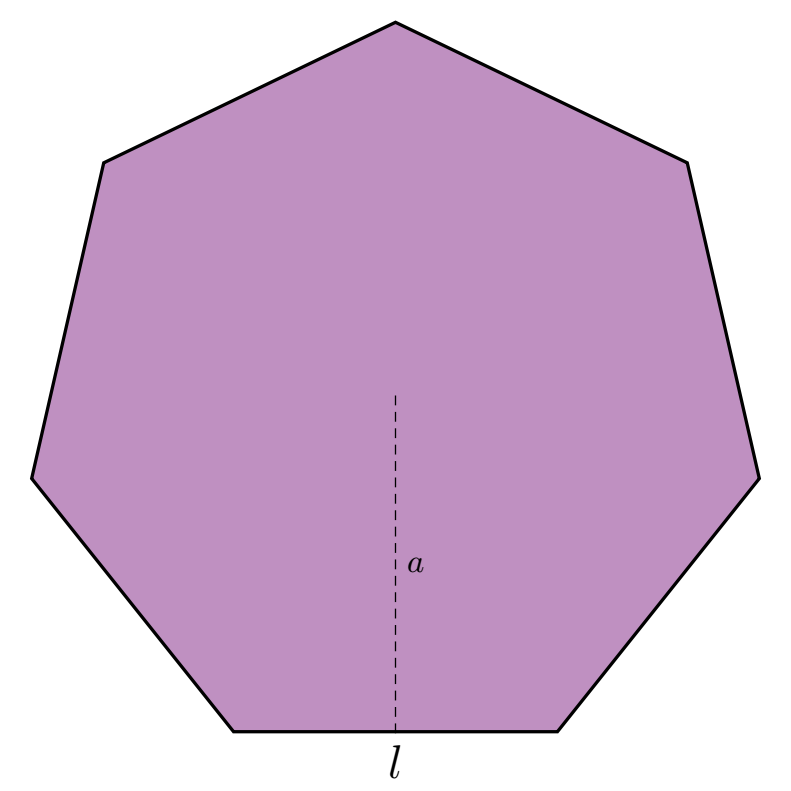
\includegraphics[width=0.9\linewidth]{mexmat00005.png}\\
                        Perímetro: \fillin[][0.3in] \quad Área: \fillin[][0.3in]

                        \begin{solutionbox}{2cm}
                        \end{solutionbox}

                        \part Si la base mayor del trapecio mide 33, su base menor 12 y su altura 14.
                        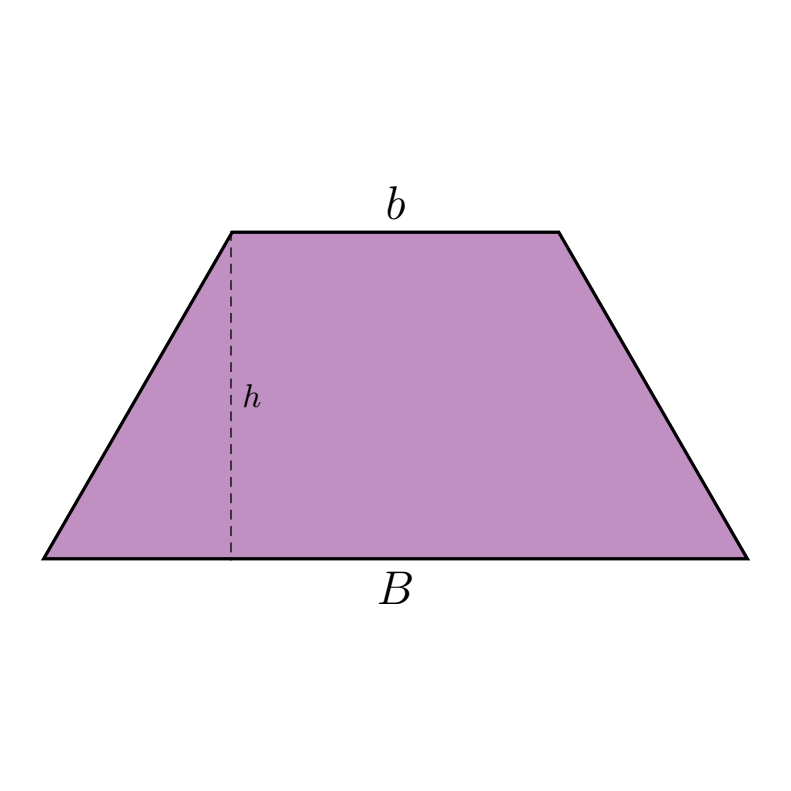
\includegraphics[width=0.9\linewidth]{mexmat00006.png}\\
                        Perímetro: \fillin[][0.3in] \quad Área: \fillin[][0.3in]

                        \begin{solutionbox}{2cm}
                        \end{solutionbox}

                        \part Si el lado del polígono mide 25 y su apotema 18.2.
                        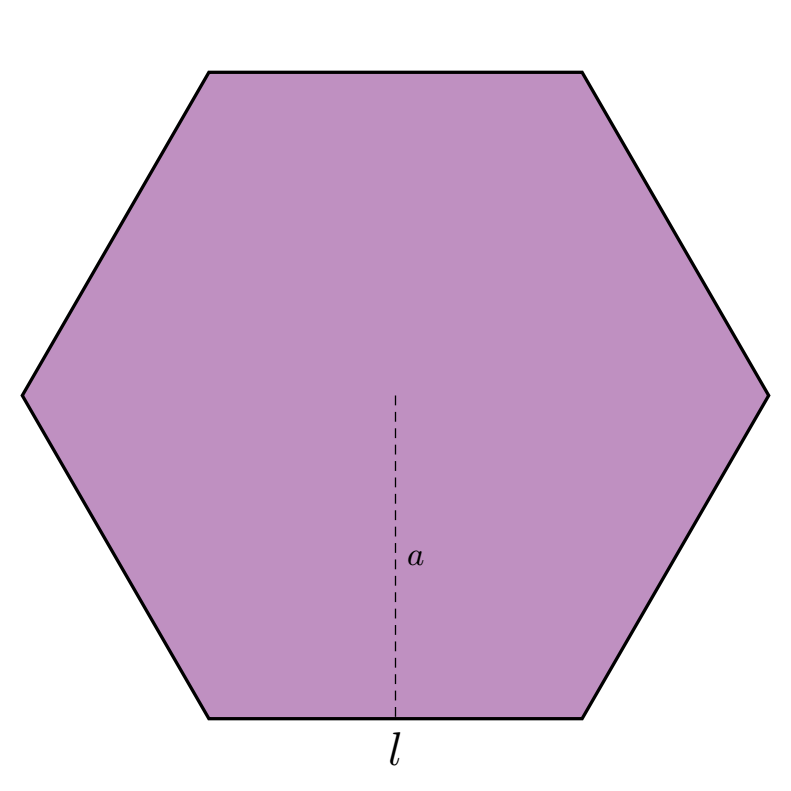
\includegraphics[width=0.9\linewidth]{mexmat00007.png}\\
                        Perímetro: \fillin[][0.3in] \quad Área: \fillin[][0.3in]

                        \begin{solutionbox}{2cm}
                        \end{solutionbox}
                  \end{parts}
            \end{multicols}
      }

      % \newpage

      % \subsection*{\ifprintanswers{Área lateral y total}\else{}\fi}
      % \subsection*{\ifprintanswers{Volumen}\else{}\fi}

      \question[6]{Calcula el volumen, el área lateral y el área total de las siguientes figuras:
            \begin{multicols}{2}
                  \begin{parts}
                        \part 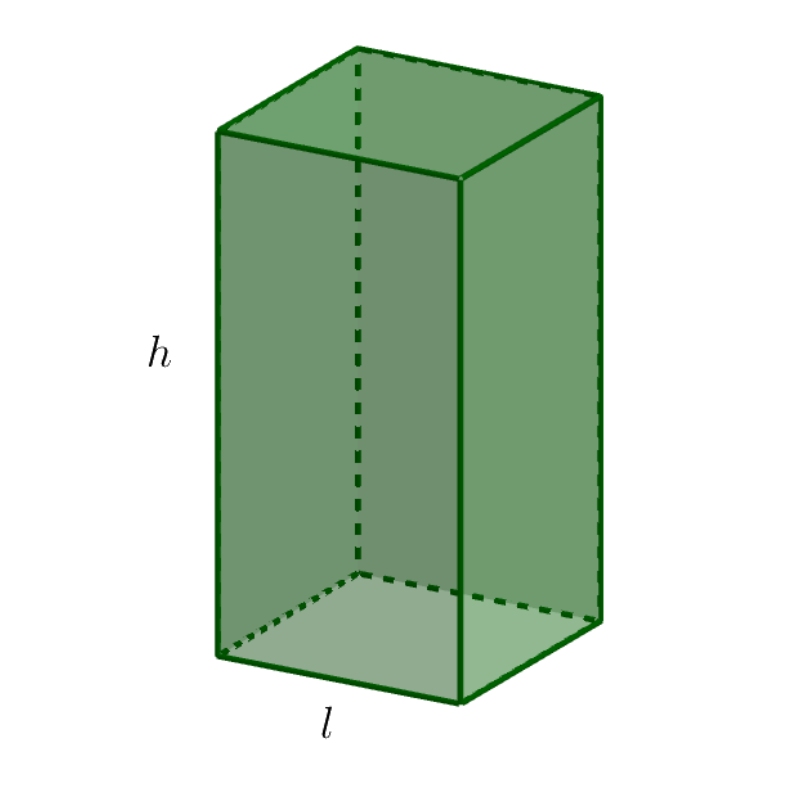
\includegraphics[width=0.65\linewidth]{mexmat00008.png}\\
                        Prisma cuyos lados "l" de la base miden 15 cm y la altura "h" mide 24 cm.\\

                        Área Lateral: \fillin[][0in]

                        \begin{solutionbox}{1cm}
                        \end{solutionbox}

                        Área Total: \fillin[][0in]

                        \begin{solutionbox}{1cm}
                        \end{solutionbox}

                        Volumen: \fillin[][0in]

                        \begin{solutionbox}{1cm}
                        \end{solutionbox}

                        \part 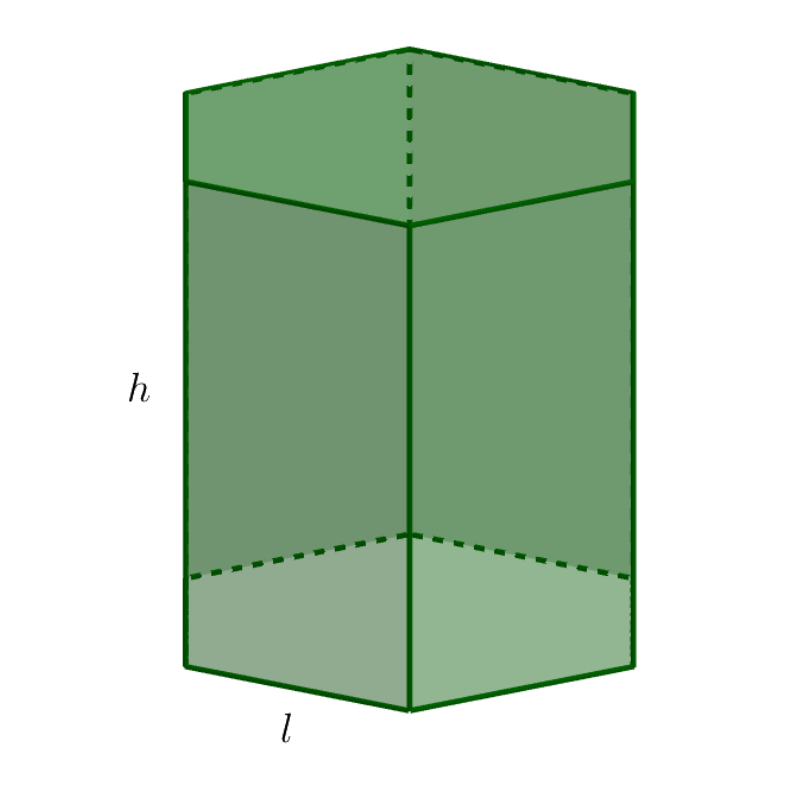
\includegraphics[width=0.65\linewidth]{mexmat00009.png}\\
                        Prisma cuyos lados "l" de la base miden 15.2 cm, el apotema mide 12.5 y la altura "h" mide 41.4 cm.\\

                        Área Lateral: \fillin[][0in]

                        \begin{solutionbox}{1cm}
                        \end{solutionbox}

                        Área Total: \fillin[][0in]

                        \begin{solutionbox}{1cm}
                        \end{solutionbox}

                        Volumen: \fillin[][0in]

                        \begin{solutionbox}{1cm}
                        \end{solutionbox}
                  \end{parts}
            \end{multicols}
      }

      % \subsection*{\ifprintanswers{Resolución de problemas}\else{}\fi}

      % \question[6]{Resuelve los siguientes problemas:

      %     \begin{multicols}{3}
      %         \begin{parts}
      %             \part
      %             \begin{solutionbox}{2cm}
      %             \end{solutionbox}
      %             \part Ernesto compró 5 sandias, si pagó un total de 120 pesos por todas, ¿cuál es el costo de una sandia?
      %             \begin{solutionbox}{2cm}
      %             \end{solutionbox}
      %             \part Si al doble de un número le restamos 19 obtenemos 61, ¿qué número es?
      %             \begin{solutionbox}{2cm}
      %             \end{solutionbox}
      %         \end{parts}
      %     \end{multicols}
      % }
\end{questions}
\end{document}